\documentclass[a4paper,11pt]{article}

\usepackage[T1]{fontenc}

\usepackage[utf8]{inputenc}

\usepackage[italian]{babel}

\usepackage{graphicx}

\usepackage{indentfirst}

\usepackage{amsmath,amssymb}

\usepackage{enumitem} 

\newcommand{\virgolette}[1]{``#1''}

\usepackage[margin=1in]{geometry} %Smaller margins

\usepackage{lmodern} %Vector PDF

\usepackage{siunitx}

\usepackage{xcolor}

\usepackage{colortbl}

\usepackage{multirow}

\usepackage{rotating}

\usepackage{booktabs}

\usepackage{longtable}

\usepackage{graphicx}
\graphicspath{ {../../Immagini/} }

\usepackage{wrapfig}

\usepackage{siunitx} % Per unit� di misura in generale e la corretta rappresentazione dei numeri.

\usepackage{gensymb} % Per il simbolo di gradi

\begin{document}
	\section{Iter sperimentale}
	L'iter sperimentale può essere diviso nelle singole procedure utilizzate per compiere le diverse misure che erano l'obbiettivo dell'esperienza.
	
	\begin{wrapfigure}{r}{0.5\textwidth}
		\vspace{-2.2cm}
		\caption{Fotografia dell'apparato sperimentale}
		\vspace{0.2cm}
		\centering
		\label{apparato}
		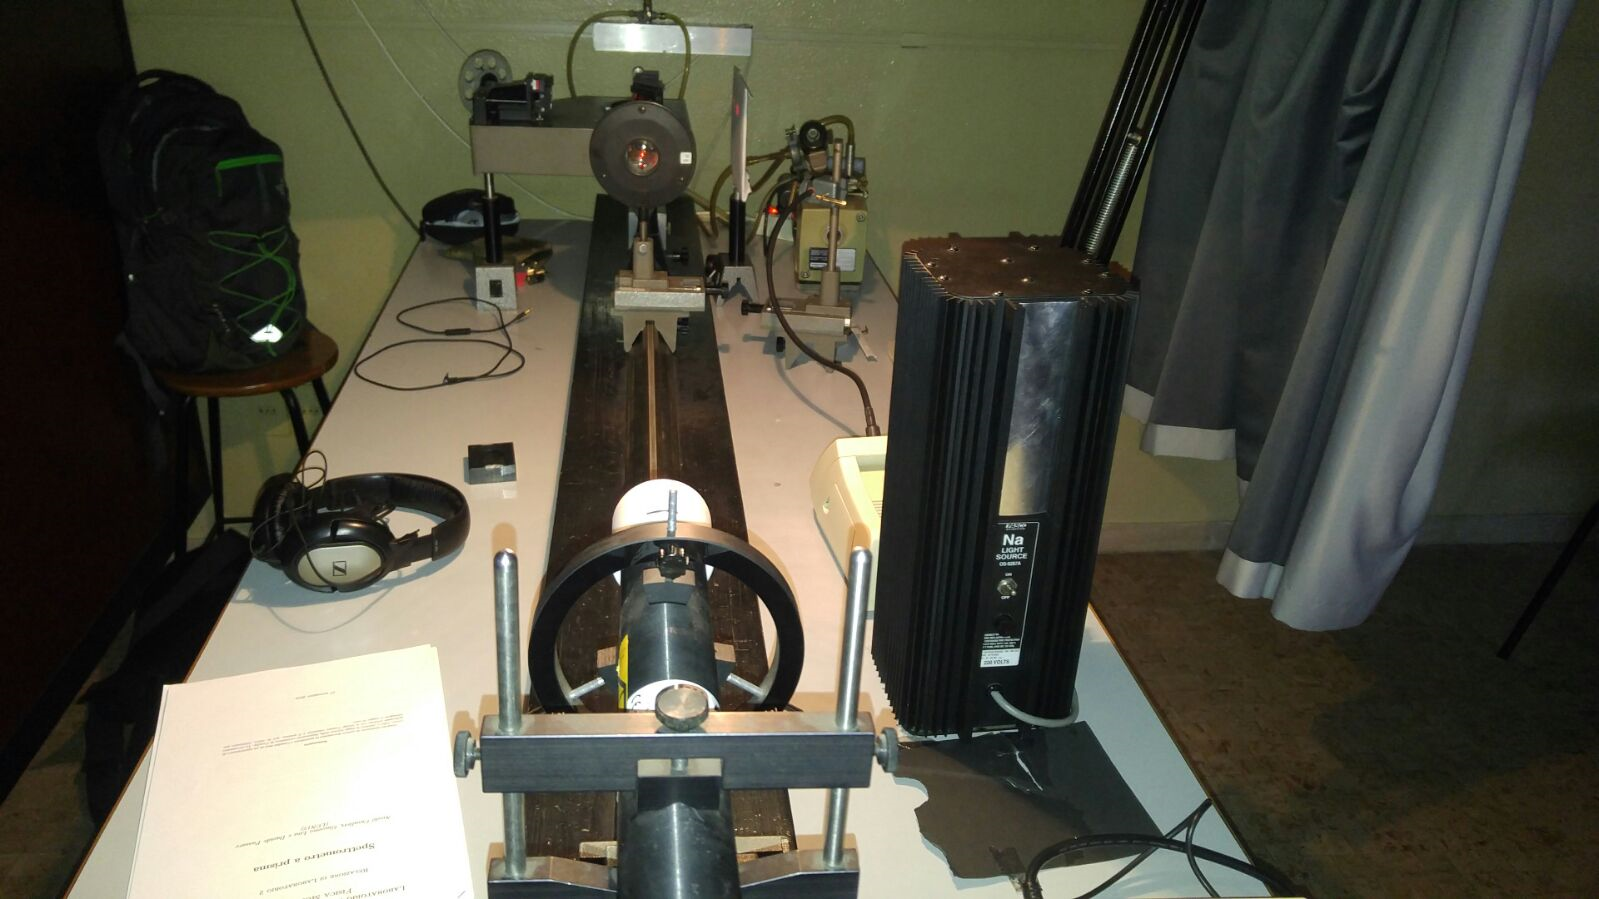
\includegraphics[width=0.48\textwidth]{apparato}
		\vspace{-1cm}
	\end{wrapfigure}
	
	\subsection{Lunghezza d'onda del laser}
	La prima parte dell'esperienza richiedeva una misura della lunghezza d'onda del laser. Questa operazione era sensata poiché il laser è un fascio di luce monocromatico e quindi dotato di una sola lunghezza d'onda.
	
	\subsubsection{Calibrazione dello specchio fisso}\label{calib}
	Per la misura della lunghezza d'onda del raggio laser è stata necessaria una calibrazione dell'interferometro volta al rendere lo specchio fisso perfettamente perpendicolare allo specchio mobile. Questo è stato fatto in due fasi. Per avere una condizione di perpendicolarità entro qualche primo è stata tolta la lente convergente. Sullo schermo si vedevano dei punti luminosi\footnote{Questi erano causati non interferenza ma da riflessioni \emph{parassite} dovute a riflessioni non volute degli innumerevoli specchi e lenti presenti nell'apparato.} ma i due corrispondenti alle riflessioni principali erano chiaramente distinguibili. Attraverso le viti dello specchio fisso si è quindi corretta la posizione dello specchio fino a quando i due punti luminosi non erano sovrapposti. Si è quindi proceduto inserendo tra la sorgente luminosa e il \emph{beam splitter}  la lente convergente. Sullo schermo erano quindi visibili i punti più luminosi sovrapposti e ingranditi. Attraverso un ulteriore aggiustamento dello specchio fisso si è potuti arrivare ad una condizione di quasi perfetta perpendicolarità, arrivando a vedere le frange di interferenza.
	
	\subsubsection{Misura}
	La misura della lunghezza d'onda ha sfruttato la possibilità di poter variare la posizione dello specchio mobile e quindi la differenza di cammino ottico dei raggi di luce. In questo modo era possibile controllare l'interferenza dei raggi luminosi e farli interferire in modo costruttivo o distruttivo. In particolare, affinché una frangia scura sullo schermo (corrispondente all'interferenza distruttiva) sostituisca una luminosa (interferenza costruttiva) è necessario spostare lo specchio di 
	\[ \Delta x = \dfrac{\lambda}{4n_a} \]
	dove $ \lambda $ è la lunghezza d'onda e $ n_a $ è l'indice di rifrazione dell'aria. Inoltre affinché una frangia chiara sostituisse una scura era necessario un ulteriore spostamento $ \Delta x $, da cui, per far si che una frangia chiara venga sostituita dalla successiva era necessario uno spostamento di $ 2\Delta x $.
	
	Poichè però la lunghezza d'onda era poco più grande della sensibilità dello strumento (la sensibilità era di $ \SI{0.2}{\micro\meter} $ mentre la lunghezza d'onda era dell'ordine di grandezza di $ \SI{100}{\nano\meter} $) per ottenere una misura con un errore accettabile era necessario far scorrere molte (circa $ \num{200} $) frange e dividere lo spostamento finale per il numero di frange viste. Si otteneva così che:
	\begin{equation}\label{\lambda}
		contenuto...
	\end{equation}
\end{document}
